\documentclass[border=4pt]{standalone}
\usepackage{tikz}
\usetikzlibrary{arrows.meta}
\begin{document}
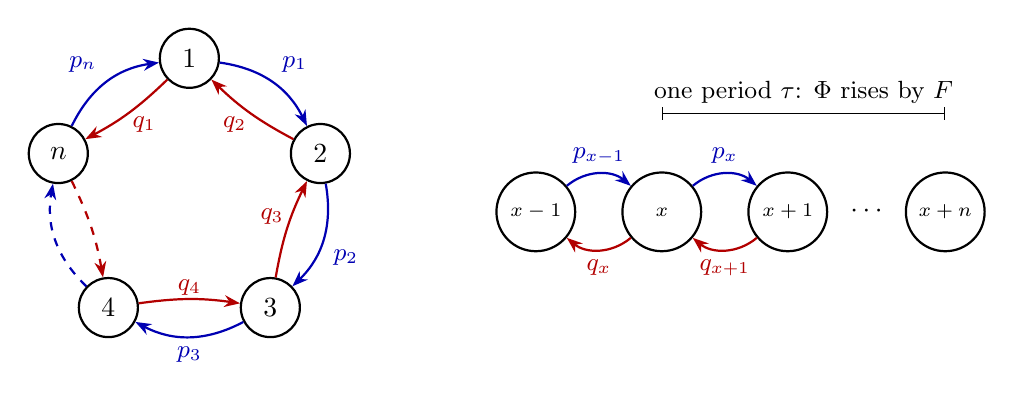
\begin{tikzpicture}[>={Stealth[length=2mm]},
  st/.style={circle,draw,thick,minimum size=7.5mm,inner sep=0pt,fill=white}]
  \def\R{1.75}
  \foreach \k/\lab in {0/1,1/2,2/3,3/4,4/n} {
    \node[st] (s\k) at ({90-72*\k}:\R) {$\lab$};
  }
  % forward arrows (outside), backward arrows (inside)
  \foreach \a/\b/\pl/\ql in {0/1/p_1/q_2,1/2/p_2/q_3,2/3/p_3/q_4,4/0/p_n/q_1} {
    \draw[->,thick,blue!70!black] (s\a) to[bend left=28] node[midway,auto,font=\small] {$\pl$} (s\b);
    \draw[->,thick,red!70!black] (s\b) to[bend left=8] node[midway,auto,font=\small,inner sep=1pt] {$\ql$} (s\a);
  }
  \draw[->,thick,blue!70!black,dashed] (s3) to[bend left=28] (s4);
  \draw[->,thick,red!70!black,dashed] (s4) to[bend left=8] (s3);
  % lifted walk
  \begin{scope}[xshift=4.4cm,yshift=-0.2cm]
    \node[st,minimum size=10mm,font=\scriptsize] (la) at (0,0) {$x-1$};
    \node[st,minimum size=10mm,font=\scriptsize] (lb) at (1.6,0) {$x$};
    \node[st,minimum size=10mm,font=\scriptsize] (lc) at (3.2,0) {$x+1$};
    \node[st,minimum size=10mm,font=\scriptsize] (ld) at (5.2,0) {$x+n$};
    \draw[->,thick,blue!70!black] (la) to[bend left=40] node[above,font=\small] {$p_{x-1}$} (lb);
    \draw[->,thick,blue!70!black] (lb) to[bend left=40] node[above,font=\small] {$p_x$} (lc);
    \draw[->,thick,red!70!black] (lb) to[bend left=40] node[below,font=\small] {$q_x$} (la);
    \draw[->,thick,red!70!black] (lc) to[bend left=40] node[below,font=\small] {$q_{x+1}$} (lb);
    \node at (4.2,0) {$\cdots$};
    \draw[|-|,thin] (1.6,1.25) -- node[above,font=\small] {one period $\tau$: $\Phi$ rises by $F$} (5.2,1.25);
  \end{scope}
\end{tikzpicture}
\end{document}
